\documentclass[11pt]{article}
\usepackage[a4paper,margin=18mm]{geometry}
\usepackage{fontspec}
\setmainfont{Latin Modern Roman}
\usepackage{amsmath,amssymb,amsthm,amscd,graphicx,color}
\usepackage{xurl}
\usepackage[unicode,hidelinks]{hyperref}
\allowdisplaybreaks
\setlength\emergencystretch{3em}




%\usepackage{showkeys}

\newcommand{\bs}{\baselineskip}
\newcommand{\yn}{\mathbb{Y}}
\newcommand{\yc}{\Yvcentermath1}
\newcommand{\mb}{\mbox{}}
% Independently written editorial renderer, restricted to the thirteen author calls.
% No bundled young.sty implementation is copied or loaded.
\usepackage{tikz}
\newcommand{\SigmaYoungOne}{\raisebox{-4.5pt}{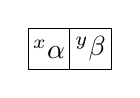
\begin{tikzpicture}[x=15pt,y=-15pt,baseline=(current bounding box.south),line width=.4pt]
\draw (0,0) rectangle (1,1);\node[inner sep=0pt] at (0.5,0.5) {\normalsize ${}^x\alpha$};
\draw (1,0) rectangle (2,1);\node[inner sep=0pt] at (1.5,0.5) {\normalsize ${}^y\beta$};
\end{tikzpicture}}}
\newcommand{\SigmaYoungTwo}{\raisebox{-12.0pt}{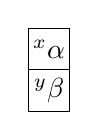
\begin{tikzpicture}[x=15pt,y=-15pt,baseline=(current bounding box.south),line width=.4pt]
\draw (0,0) rectangle (1,1);\node[inner sep=0pt] at (0.5,0.5) {\normalsize ${}^x\alpha$};
\draw (0,1) rectangle (1,2);\node[inner sep=0pt] at (0.5,1.5) {\normalsize ${}^y\beta$};
\end{tikzpicture}}}
\newcommand{\SigmaYoungThree}{\raisebox{-21.0pt}{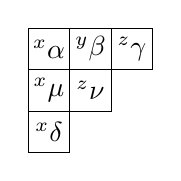
\begin{tikzpicture}[x=15pt,y=-15pt,baseline=(current bounding box.south),line width=.4pt]
\draw (0,0) rectangle (1,1);\node[inner sep=0pt] at (0.5,0.5) {\normalsize ${}^x\alpha$};
\draw (1,0) rectangle (2,1);\node[inner sep=0pt] at (1.5,0.5) {\normalsize ${}^y\beta$};
\draw (2,0) rectangle (3,1);\node[inner sep=0pt] at (2.5,0.5) {\normalsize ${}^z\gamma$};
\draw (0,1) rectangle (1,2);\node[inner sep=0pt] at (0.5,1.5) {\normalsize ${}^x\mu$};
\draw (1,1) rectangle (2,2);\node[inner sep=0pt] at (1.5,1.5) {\normalsize ${}^z\nu$};
\draw (0,2) rectangle (1,3);\node[inner sep=0pt] at (0.5,2.5) {\normalsize ${}^x\delta$};
\end{tikzpicture}}}
\newcommand{\SigmaYoungFour}{\raisebox{-21.0pt}{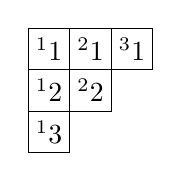
\begin{tikzpicture}[x=15pt,y=-15pt,baseline=(current bounding box.south),line width=.4pt]
\draw (0,0) rectangle (1,1);\node[inner sep=0pt] at (0.5,0.5) {\normalsize ${}^1 1$};
\draw (1,0) rectangle (2,1);\node[inner sep=0pt] at (1.5,0.5) {\normalsize ${}^2 1$};
\draw (2,0) rectangle (3,1);\node[inner sep=0pt] at (2.5,0.5) {\normalsize ${}^3 1$};
\draw (0,1) rectangle (1,2);\node[inner sep=0pt] at (0.5,1.5) {\normalsize ${}^1 2$};
\draw (1,1) rectangle (2,2);\node[inner sep=0pt] at (1.5,1.5) {\normalsize ${}^2 2$};
\draw (0,2) rectangle (1,3);\node[inner sep=0pt] at (0.5,2.5) {\normalsize ${}^1 3$};
\end{tikzpicture}}}
\newcommand{\SigmaYoungFive}{\raisebox{-21.0pt}{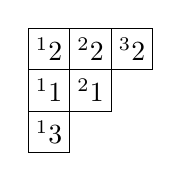
\begin{tikzpicture}[x=15pt,y=-15pt,baseline=(current bounding box.south),line width=.4pt]
\draw (0,0) rectangle (1,1);\node[inner sep=0pt] at (0.5,0.5) {\normalsize ${}^1 2$};
\draw (1,0) rectangle (2,1);\node[inner sep=0pt] at (1.5,0.5) {\normalsize ${}^2 2$};
\draw (2,0) rectangle (3,1);\node[inner sep=0pt] at (2.5,0.5) {\normalsize ${}^3 2$};
\draw (0,1) rectangle (1,2);\node[inner sep=0pt] at (0.5,1.5) {\normalsize ${}^1 1$};
\draw (1,1) rectangle (2,2);\node[inner sep=0pt] at (1.5,1.5) {\normalsize ${}^2 1$};
\draw (0,2) rectangle (1,3);\node[inner sep=0pt] at (0.5,2.5) {\normalsize ${}^1 3$};
\end{tikzpicture}}}
\newcommand{\SigmaYoungSix}{\raisebox{-12.0pt}{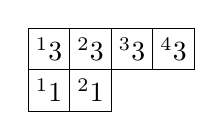
\begin{tikzpicture}[x=15pt,y=-15pt,baseline=(current bounding box.south),line width=.4pt]
\draw (0,0) rectangle (1,1);\node[inner sep=0pt] at (0.5,0.5) {\normalsize ${}^1 3$};
\draw (1,0) rectangle (2,1);\node[inner sep=0pt] at (1.5,0.5) {\normalsize ${}^2 3$};
\draw (2,0) rectangle (3,1);\node[inner sep=0pt] at (2.5,0.5) {\normalsize ${}^3 3$};
\draw (3,0) rectangle (4,1);\node[inner sep=0pt] at (3.5,0.5) {\normalsize ${}^4 3$};
\draw (0,1) rectangle (1,2);\node[inner sep=0pt] at (0.5,1.5) {\normalsize ${}^1 1$};
\draw (1,1) rectangle (2,2);\node[inner sep=0pt] at (1.5,1.5) {\normalsize ${}^2 1$};
\end{tikzpicture}}}
\newcommand{\SigmaEmptyOne}{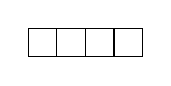
\begin{tikzpicture}[x=2.4ex,y=-2.4ex,baseline={([yshift=-.5ex]current bounding box.center)},line width=.4pt]
\draw (0,0) rectangle (1,1);
\draw (1,0) rectangle (2,1);
\draw (2,0) rectangle (3,1);
\draw (3,0) rectangle (4,1);
\end{tikzpicture}}
\newcommand{\SigmaEmptyTwo}{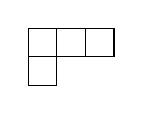
\begin{tikzpicture}[x=2.4ex,y=-2.4ex,baseline={([yshift=-.5ex]current bounding box.center)},line width=.4pt]
\draw (0,0) rectangle (1,1);
\draw (1,0) rectangle (2,1);
\draw (2,0) rectangle (3,1);
\draw (0,1) rectangle (1,2);
\end{tikzpicture}}
\newcommand{\SigmaEmptyThree}{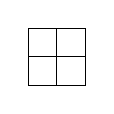
\begin{tikzpicture}[x=2.4ex,y=-2.4ex,baseline={([yshift=-.5ex]current bounding box.center)},line width=.4pt]
\draw (0,0) rectangle (1,1);
\draw (1,0) rectangle (2,1);
\draw (0,1) rectangle (1,2);
\draw (1,1) rectangle (2,2);
\end{tikzpicture}}
\newcommand{\SigmaEmptyFour}{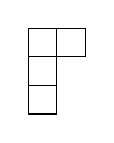
\begin{tikzpicture}[x=2.4ex,y=-2.4ex,baseline={([yshift=-.5ex]current bounding box.center)},line width=.4pt]
\draw (0,0) rectangle (1,1);
\draw (1,0) rectangle (2,1);
\draw (0,1) rectangle (1,2);
\draw (0,2) rectangle (1,3);
\end{tikzpicture}}
\newcommand{\SigmaEmptyFive}{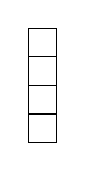
\begin{tikzpicture}[x=2.4ex,y=-2.4ex,baseline={([yshift=-.5ex]current bounding box.center)},line width=.4pt]
\draw (0,0) rectangle (1,1);
\draw (0,1) rectangle (1,2);
\draw (0,2) rectangle (1,3);
\draw (0,3) rectangle (1,4);
\end{tikzpicture}}
\newcommand{\SigmaEmptySix}{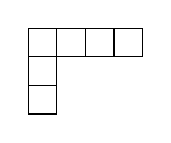
\begin{tikzpicture}[x=2.4ex,y=-2.4ex,baseline={([yshift=-.5ex]current bounding box.center)},line width=.4pt]
\draw (0,0) rectangle (1,1);
\draw (1,0) rectangle (2,1);
\draw (2,0) rectangle (3,1);
\draw (3,0) rectangle (4,1);
\draw (0,1) rectangle (1,2);
\draw (0,2) rectangle (1,3);
\end{tikzpicture}}
\newcommand{\SigmaEmptySeven}{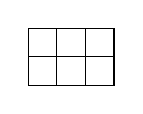
\begin{tikzpicture}[x=2.4ex,y=-2.4ex,baseline={([yshift=-.5ex]current bounding box.center)},line width=.4pt]
\draw (0,0) rectangle (1,1);
\draw (1,0) rectangle (2,1);
\draw (2,0) rectangle (3,1);
\draw (0,1) rectangle (1,2);
\draw (1,1) rectangle (2,2);
\draw (2,1) rectangle (3,2);
\end{tikzpicture}}
\ExplSyntaxOn
\msg_new:nnn{sigmafinite}{unknown}{Unsupported~editorial~Young~diagram~call.}
\cs_new_protected:Npn\sigma_check:nn#1#2{\tl_set:Nx\l_tmpa_tl{\tl_to_str:n{#1}}\tl_set:Nx\l_tmpb_tl{\tl_to_str:n{#2}}\regex_replace_all:nnN{\s+}{}\l_tmpa_tl\regex_replace_all:nnN{\s+}{}\l_tmpb_tl\tl_if_eq:NNF\l_tmpa_tl\l_tmpb_tl{\msg_fatal:nn{sigmafinite}{unknown}}}
\int_new:N\g_sigma_young_int
\int_new:N\g_sigma_empty_int
\int_new:N\g_sigma_yng_int
\NewDocumentCommand{\YoungTab}{O{0} O{} m}{\int_gincr:N\g_sigma_young_int\int_case:nnF{\g_sigma_young_int}{
{1}{\str_if_eq:eeF{#1}{-0.3}{\msg_fatal:nn{sigmafinite}{unknown}}\tl_if_eq:nnF{#2}{\normalsize}{\msg_fatal:nn{sigmafinite}{unknown}}\sigma_check:nn{#3}{ {{}^x\alpha,{}^y\beta} }\SigmaYoungOne}{2}{\str_if_eq:eeF{#1}{-0.8}{\msg_fatal:nn{sigmafinite}{unknown}}\tl_if_eq:nnF{#2}{\normalsize}{\msg_fatal:nn{sigmafinite}{unknown}}\sigma_check:nn{#3}{ {{}^x\alpha}{{}^y\beta} }\SigmaYoungTwo}{3}{\str_if_eq:eeF{#1}{-1.4}{\msg_fatal:nn{sigmafinite}{unknown}}\tl_if_eq:nnF{#2}{\normalsize}{\msg_fatal:nn{sigmafinite}{unknown}}\sigma_check:nn{#3}{ {{}^x\alpha,{}^y\beta,{}^z\gamma} {{}^x\mu,{}^z\nu } {{}^x\delta }}\SigmaYoungThree}{4}{\str_if_eq:eeF{#1}{-1.4}{\msg_fatal:nn{sigmafinite}{unknown}}\tl_if_eq:nnF{#2}{\normalsize}{\msg_fatal:nn{sigmafinite}{unknown}}\sigma_check:nn{#3}{ {{}^1 1,{}^2 1,{}^3 1} {{}^1 2,{}^2 2 } {{}^1 3 }}\SigmaYoungFour}{5}{\str_if_eq:eeF{#1}{-1.4}{\msg_fatal:nn{sigmafinite}{unknown}}\tl_if_eq:nnF{#2}{\normalsize}{\msg_fatal:nn{sigmafinite}{unknown}}\sigma_check:nn{#3}{ {{}^1 2,{}^2 2,{}^3 2} {{}^1 1,{}^2 1 } {{}^1 3 }}\SigmaYoungFive}{6}{\str_if_eq:eeF{#1}{-0.8}{\msg_fatal:nn{sigmafinite}{unknown}}\tl_if_eq:nnF{#2}{\normalsize}{\msg_fatal:nn{sigmafinite}{unknown}}\sigma_check:nn{#3}{ {{}^1 3,{}^2 3,{}^3 3, {}^4 3 } {{}^1 1,{}^2 1 } }\SigmaYoungSix}}{\msg_fatal:nn{sigmafinite}{unknown}}}
\NewDocumentCommand{\Yvcentermath}{m}{\str_if_eq:eeF{#1}{1}{\msg_fatal:nn{sigmafinite}{unknown}}}
\NewDocumentCommand{\young}{r()}{\int_gincr:N\g_sigma_empty_int\int_case:nnF{\g_sigma_empty_int}{
{1}{\tl_if_eq:nnF{#1}{\mb\mb\mb\mb}{\msg_fatal:nn{sigmafinite}{unknown}}\SigmaEmptyOne}{2}{\tl_if_eq:nnF{#1}{\mb\mb\mb,\mb}{\msg_fatal:nn{sigmafinite}{unknown}}\SigmaEmptyTwo}{3}{\tl_if_eq:nnF{#1}{\mb\mb,\mb\mb}{\msg_fatal:nn{sigmafinite}{unknown}}\SigmaEmptyThree}{4}{\tl_if_eq:nnF{#1}{\mb\mb,\mb,\mb}{\msg_fatal:nn{sigmafinite}{unknown}}\SigmaEmptyFour}{5}{\tl_if_eq:nnF{#1}{\mb,\mb,\mb,\mb}{\msg_fatal:nn{sigmafinite}{unknown}}\SigmaEmptyFive}}{\msg_fatal:nn{sigmafinite}{unknown}}}
\NewDocumentCommand{\yng}{r()}{\int_gincr:N\g_sigma_yng_int\int_case:nnF{\g_sigma_yng_int}{
{1}{\tl_if_eq:nnF{#1}{4,1,1}{\msg_fatal:nn{sigmafinite}{unknown}}\SigmaEmptySix}
{2}{\tl_if_eq:nnF{#1}{3,3}{\msg_fatal:nn{sigmafinite}{unknown}}\SigmaEmptySeven}
}{\msg_fatal:nn{sigmafinite}{unknown}}}
\AtEndDocument{\int_compare:nNnF{\g_sigma_young_int}={6}{\msg_fatal:nn{sigmafinite}{unknown}}\int_compare:nNnF{\g_sigma_empty_int}={5}{\msg_fatal:nn{sigmafinite}{unknown}}\int_compare:nNnF{\g_sigma_yng_int}={2}{\msg_fatal:nn{sigmafinite}{unknown}}}
\ExplSyntaxOff

\begin{document}
\begin{center}\Large Strict dominance ordering and unique minimal-energy multiplets at fixed particle number for finite open SU(N) extended Hubbard chains with N at least three, positive hopping, exchange and pair hopping, and real number-dependent potential\end{center}
\noindent\textbf{Stable ID:} 2753\par
\noindent\textbf{Authors:} Tigran Hakobyan\par
\noindent\textbf{Original work:} Ordering of Energy Levels for Extended SU(N) Hubbard Chain\par
\noindent\textbf{Version:} Official SIGMA 6 (2010) article 024, DOI 10.3842/SIGMA.2010.024; journal PDF and native TeX acquired 2026-10-01, exact bytes pinned by SHA256\par
\noindent\textbf{Selected task scope:} Finite open chain with L sites and N>=\allowbreak{}3 fermion flavors, the exact Hamiltonian(1), all t\_x,J\_x,K\_x>0 and arbitrary real V(n\_1,...,n\_L). Fix total particle number M. For each realized U(N) Young type Y with M boxes, at most N rows and first row<=\allowbreak{}L, its sector minimum consists of one irreducible multiplet (ordinary SU(N) dimension degeneracy allowed). If two such diagrams satisfy strict dominance Y2>Y1, then E(Y2)>E(Y1). No ordering across different M or incomparable diagrams, and no periodic-boundary extension.\par
\noindent\textbf{Difficulty:} H2: Perron-Frobenius positivity alone does not identify which irreducible flavor representation contains a many-fermion sector minimum. The author constructs a fermionic sign basis for hopping, exchange and pair hopping, and a compact trial configuration whose row symmetrization and column antisymmetrization isolate one Young type. Positive overlap and uniqueness then identify the relative ground multiplet, and a shared-weight comparison proves strict energy ordering under diagram dominance.\par
\noindent\textbf{Editorial boundary note (not author text):} The full original Section5 energy-ordering and multiplet-uniqueness conclusion is retained for the finite open-chain Hamiltonian, positive hopping/exchange/pair-hopping and arbitrary occupation-number potential. The full fermionic nonpositive basis, connectivity/positivity, compact trial-state Young-type identification and shared-weight strict dominance comparison are bundled into one main outcome. The Perron-Frobenius theorem and standard unitary/Young representation facts remain explicitly cited foundations. SU(N) representation degeneracy is preserved; later total-ground-state and continuum conclusions are unselected.\par
\noindent\textbf{Source:} \url{https://sigma-journal.com/2010/024/}\quad DOI: \url{https://doi.org/10.3842/SIGMA.2010.024}\par
\noindent\textbf{License and attribution:} Copyright retained by the named authors. Published by SIGMA under CC BY 4.0: \url{https://creativecommons.org/licenses/by/4.0/}. Source: \url{https://sigma-journal.com/about.html}. Adaptation consists of standalone excerpt formatting, cover and numbering restoration; original author language and mathematical text are retained.\par
\noindent\textbf{Editorial symbol notice (not author text):} Original scalar completeness/diagonal displays use lowercase n where the flavor count is denoted N elsewhere. These occupation-number diagonal terms are explicitly absorbed into arbitrary V in the authored proof; the exact source Hamiltonian and all source formulas remain unchanged. Sector uniqueness means one multiplet, not a simple eigenvalue after discarding SU(N) degeneracy.\par
\noindent\textbf{Typesetting adaptation (not author text):} The thirteen retained Young-diagram calls are rendered by an independently written editorial TikZ renderer restricted to six exact labeled tableaux, five stated empty four-box partitions and two stated empty six-box shapes. Exact author arguments and invocation counts are checked; unknown calls are rejected. No bundled third-party style implementation is copied. Original cells, row boundaries, entries, upper-left site superscripts and equation attachment are retained.\par
\medskip\hrule\medskip\noindent\textbf{Author text begins below.}\par
\setcounter{section}{1}
\setcounter{subsection}{0}
\setcounter{subsubsection}{0}
\setcounter{equation}{0}
% Original source lines 126--541
\section[$SU(N)$ symmetric fermionic chain]{$\boldsymbol{SU(N)}$ symmetric fermionic chain}\label{section2}

Consider the f\/inite-size $SU(N)$ symmetric extended Hubbard chain described by the Hamiltonian
\begin{gather}
H=\sum_{x,\alpha} -t_x\big( c^+_{x+1,\alpha}c_{x,\alpha} + c^+_{x,\alpha}c_{x+1,\alpha}\big)
+  V(n_1,\dots,n_L) + \sum_{x,a} J_x\ T_x^a  T_{x+1}^a\nonumber
\\
\phantom{H=}{}- \sum_{x,\alpha>\beta} K_x\big(
c^+_{x+1,\alpha} c^+_{x+1,\beta} c_{x,\beta} c_{x,\alpha}
+ c^+_{x,\alpha} c^+_{x,\beta} c_{x+1,\beta} c_{x+1,\alpha}\big),\label{H}
\end{gather}
where the open boundary conditions $\left(\sum_x=\sum_{x=1}^{L-1}\right)$ are supposed.
The coef\/f\/icients $t_x$, $J_x$ and~$K_x$ are positive and dependent on the site~$x$.
There are $N$ dif\/ferent f\/lavors of fermions, which are numbered by $\alpha$.
The fermion  creation  $c^+_{x,\alpha}$ and annihilation  $c_{x,\alpha}$ operators
obey the standard  anticommutation relations.

In the above Hamiltonian, $n_x=\sum_{\alpha}n_{x,\alpha}=\sum_{\alpha} c^+_{x,\alpha}c_{x,\alpha}$
is the fermion number at the $x$-th site.
The form of the potential $V(n_1,\dots,n_L)$ does not matter, the
only restriction is that it depends only on the local fermion numbers.
The Hubbard potential is a particular case
$V=U/2\sum_x n_x^2$.
It is equivalent, up to the total particle number,
to $U\sum_{x,\alpha>\beta}n_{x,\alpha}n_{x,\beta}$.


The third term is the Heisenberg interaction of $SU(N)$ spins (f\/lavors) given in
the Schwinger representation
\begin{equation}
\label{schwinger}
T_x^a=\sum_{\alpha,\beta}
c_{x,\alpha}^+ \mathcal{T}^a_{\alpha\beta} c_{x,\beta}, \qquad a=1,\dots,N^2-1=\dim SU(N),
\end{equation}
where $\mathcal{T}^a_{\alpha\beta}$ are the generators of $SU(N)$ Lie
algebra in the def\/ining representation, which are  orthogonal
with respect to the trace.
 Using the completeness relation for $SU(N)$ matrices
\[
\sum_a\mathcal{T}^a_{\alpha\beta}\mathcal{T}^a_{\alpha'\beta'}=
2\delta_{\alpha\beta'} \delta_{\alpha'\beta}  -\frac{2}{n} \delta_{\alpha\beta} \delta_{\alpha'\beta'},
\]
one can rewrite this term in the following form \cite{MA89}:
\begin{gather}
\sum_{a} T_x^a  T_{x+1}^a
=
2\sum_{\alpha,\beta} c^+_{x,\alpha}  c_{x,\beta} c^+_{x+1,\beta} c_{x+1,\alpha}
- \frac{2}{n} n_x n_{x+1}\nonumber
\\
\hphantom{\sum_{a} T_x^a  T_{x+1}^a}{}=
-2\sum_{\alpha,\beta} c^+_{x,\alpha}  c_{x+1,\alpha}  c^+_{x+1,\beta} c_{x,\beta}+2n_x- \frac{2}{n} n_x n_{x+1},\label{heis}
\end{gather}
The f\/irst term above just exchanges the f\/lavors between
adjacent sites \cite{AL86}. The last two terms depend only on $n_x$ and may be included in the potential.

The last term   in \eqref{H} describes the hopping of
fermion pairs.

The Hamiltonian preserves the $U(1)$ total charge, which corresponds to the total number
of particles
\begin{equation*}
%\label{u-1}
n=\sum_{x} n_x=\sum_{x,\alpha}c_{x,\alpha}^+c_{x,\alpha}.
\end{equation*}
It is also invariant with respect to $SU(N)$ generators
\begin{equation*}
%\label{su-n}
T^a=\sum_x T^a_x= \sum_{x,\alpha,\beta}c_{x,\alpha}^+ \mathcal{T}^a_{\alpha\beta}c_{x,\beta}.
\end{equation*}
The total symmetry group is $U(N)=SU(N)\times U(1)$.
The spin-raising, spin-lowering, and Cartan generators are given by
the upper triangular, lower triangular, and diagonal
matrixes. The corresponding basis is presented below
both in the def\/ining and multi-particle representations.
\begin{equation}
\label{raising}
\big(\mathcal{F}^{\alpha\beta}\big)_{\alpha'\beta'}=\delta^\alpha_{\alpha'}\delta^\beta_{\beta'},
\qquad
F^{\alpha\beta}=\sum_x c_{x,\alpha}^+ c_{x,\beta},
\qquad
F^{\alpha\alpha}=\sum_x n_{x,\alpha}.
\end{equation}

The current system  is a $SU(N)$ generalization of the $SU(2)$ Hamiltonian,
for which the Lieb--Mattis theorem  has been established
and proven already \cite{Amb92-2}.
For the Hubbard potential, the
f\/irst three terms of the Hamiltonian \eqref{H}
correspond to the $SU(N)$ Hubbard--Heisenberg chain
introduced in~\cite{MA89}.
The $SU(4)$ system without pair-hopping and Heisenberg terms has been proven to have  nondegenerate
ground state and gapless excitations \cite{LTML04}.

Each site has $2^N$ dif\/ferent states with fermion number varying from
zero to $N$.
According to~\eqref{schwinger} or~\eqref{raising},
the one-particle states $c^+_{\alpha}|0\rangle$ form the def\/ining
representation of $U(N)$.
Similarly, due to the anticommutation of the fermionic operators,
the multi-particle states $c^+_{\alpha_1}\cdots c^+_{\alpha_k}|0\rangle $
form the $\binom{N}{k}$-dimensional antisymmetric representation.
There are two singlets ($k=0,N$), which correspond to
the vacuum $|0\rangle $ and completely f\/illed states.

In this article we follow the standard way in order to establish and prove the generalized Lieb--Mattis
theorem for the described system \cite{LM62,H07}. First, we construct a basis, in which all
nonzero of\/f-diagonal matrix elements of the Hamiltonian are negative.
Next, we conf\/ine ourselves to the subspaces, where the Hamiltonian is connected,
and due to the Perron--Frobenius theorem, the lowest-energy state
is unique and positive. Employing the positivity, we compare this state with a simple trial state
and detect in this way  the containing multiplet.
Finally, using the representation theory of $SU(N)$ group, we express the ordering
of the lowest energy levels of dif\/ferent multiplets in terms of the dominance
order of the corresponding Young diagrams.


\section{Nonpositive basis}\label{section3}

The natural basis for the Hamiltonian \eqref{H} is formed by the f\/ixed particles. The coordinates
are given by the set $\{x^\alpha\}_{\alpha=1}^N$ consisting of $N$  subsets. Each subset
\[
\{x^\alpha\}=\{x^\alpha_1,\dots,x^\alpha_{M_\alpha} | x^\alpha_1<\dots <x^\alpha_{M_\alpha}\}
\]
describes the positions of the fermions carrying the f\/lavor $\alpha$, and $M_\alpha=\#\{x^\alpha\}$
is their number. Let  $M=\sum_\alpha M_\alpha$
be the total number of particles.
It appears that for each state a sign factor can be
chosen in order to make the nonzero of\/f-diagonal elements of the Hamiltonian
negative.

First, we observe from \eqref{H} and \eqref{heis} that the of\/f-diagonal part is built of
the nearest-neighbor hoppings $c^+_{x\pm1,\alpha}c_{x,\alpha}$ and their products.
Due to the appropriate signs of the
constants $-t_x$, $-K_x$ and $J_x$,
the positive values for all nonzero  matrix elements of these hoppings
imply  the non-positive values for the of\/f-diagonal matrix elements of the Hamiltonian.
The correct sign factor is encoded in the following arrangement of the fermion creation operators:
\begin{equation}
\label{basis}
|\{x^1\},\dots,\{x^N\}\rangle =
\prod_{\alpha=1}^N (c^+_{x^\alpha_1,\alpha}c^+_{x^\alpha_2,\alpha}\cdots c^+_{x^\alpha_{M_\alpha},\alpha}) |0\rangle,
\end{equation}
where the product is taken from the left to the right. In other words, we group together the particles
of the same f\/lavor ordering them according to their position.
Due to the Fermi--Dirac statistics, the hopping term  $c^+_{x\pm1,\alpha}c_{x,\alpha}$ acts
nontrivially on the states having one and only one $\alpha$-fermion per two adjacent states.
In that case, it produces a similar state~\eqref{basis} with $c^+_{x,\alpha}$ just replaced by $c^+_{x\pm1,\alpha}$
without any additional sign factor.
Therefore, the of\/f-diagonal matrix elements of the  Hamiltonian~\eqref{H} in the above basis are non-positive.

The basis \eqref{basis} has been used before to study the degeneracy of the ground states.
It was described by Af\/f\/leck and Lieb and used for the
construction of  non-positive basis for the antiferromagnetic $SU(N)$ Heisenberg chains~\cite{AL86}.
An  explicit expression similar to \eqref{basis} was written
for the extended $t-J$ and $SU(2)$ Hubbard models in \cite{Amb92-1,Amb92-2}, where it
was applied for the proof of the Lieb--Mattis theorem.
For multicomponent $t-J$ model with $SU(N_b)\times SU(N_f)$
symmetry, the similar basis ensures the nondegeneracy of the relative ground states~\cite{sorella96}.
For $SU(4)$ Hubbard model, it has been used for the study
of ground state and the proof of the Lieb--Schultz--Mattis theorem~\cite{LTML04}.

It is interesting to extract the sign factor, which was encoded in the particular arrangement
of fermion operators in \eqref{basis}, in case of the pure Heisenberg system.
Note that the Heisenberg interaction preserves the number of particles on each site. Therefore, it
may be restricted to smaller subspace, where each site contains only one of $N-1$ fundamental
(antisymmetric) representations of $SU(N)$. It is easy to express the basis \eqref{basis}
in terms of the usual Ising basis of the Heisenberg model. Set, for the simplicity, one fermion per site,
which corresponds to the def\/ining $N$-dimensional representation. Then the usual Ising (Potts) basis is
\begin{equation}
\label{ising}
|\alpha_1,\dots,\alpha_L\rangle =c^+_{1,\alpha_1}c^+_{2,\alpha_2}\cdots c^+_{L,\alpha_L} |0\rangle.
\end{equation}
The Heisenberg exchange \eqref{heis} acts on these states as
\[
\sum_a T^a_xT^a_{x+1}=2P_{x,x+1}-\frac{2}{n},
\]
where $P_{x,y}$ is the permutation of two sites. The states \eqref{basis} can be obtained by
an appropriate rearrangement of the states \eqref{ising}. Since the fermions of the same f\/lavor
are already ordered by coordinates in \eqref{basis}, we get:
\[
|\{x^1\},\dots,\{x^N\}\rangle = (-1)^{p_{\alpha_1\dots\alpha_L}}
|\alpha_1,\dots,\alpha_L\rangle,
\qquad
p_{\alpha_1\dots \alpha_L} =  \{\, \#(x<y) \; | \; \alpha_x>\alpha_y\, \}.
\]
Here $p_{\alpha_1\dots \alpha_L}$ is the number of inversions in the sequence.
The nonpositive basis in this form have  been used in the study of Heisenberg chains with
higher symmetries \cite{H04,Li01}.

Note that for the systems with ref\/lection symmetry, there is
another approach referred as a ref\/lection positivity.
It can be applied for more general class of systems, like frustrated spin models
\cite{Lieb89,LS99,Shen98}. The spin f\/lip on the half of the lattice is performed
in order to construct a new basis (distinct from \eqref{basis}) from the usual one.
The ground state wavefunction becomes positive in the new
basis. The method is problematic for higher rank $ SU(N)$  spins, since most of
the multiplets, including the def\/ining one, are not invariant under the ref\/lection.
As a result, one must either use the ref\/lected (conjugate)
representations for the half of the lattice, or conf\/ine itself to
self-conjugate ones, which are not the cases considered in this article.



\section{Relative ground states}\label{section4}

The Hamiltonian is invariant on any $M_\alpha$-subspace, which is made up of the basic states~\eqref{basis} with the same number of fermions of each type. It can be considered also as
a weight subspace under the $U(N)$ action.
The weight is given by  the set $\{M_\alpha\}_{\alpha=1}^N$ composed of
the eigenvalues of the diagonal generators from \eqref{raising}.
Note that according to the Fermi--Dirac statistics, the volume  of the chain must be large
enough in order to contain all particles:
\begin{equation}
\label{size}
L\ge\max_{1\le\alpha\le N} M_\alpha.
\end{equation}
This is the condition of the existence of $M_\alpha$-subspace for the $L$-size chain.

It is easy to see that any two basic states from the same subspace
are connected by the kinetic terms of the Hamiltonian.
Then, according to the Perron--Frobenius theorem~\cite{Lancaster},
\begin{itemize}\itemsep=0pt
\item
The relative ground state of the
Hamiltonian in any $M_\alpha$-subspace is unique, and its all coef\/f\/icients
in the basis \eqref{basis} are straightly positive:
\begin{equation}
\label{rgs}
\Omega_{M_1\dots M_N}=\sum_{\substack{\{x^1\},\dots,\{x^N\}\\ \#\{x^\alpha\}=M_\alpha}}
\omega_{\{x^1\}\dots\{x^N\}} |\{x^1\},\dots,\{x^N\}\rangle,
\qquad  \omega_{\{x^1\}\dots\{x^N\}} >0.
\end{equation}
\end{itemize}

The positivity can be used in order to trace the type of the $U(N)$
multiplet, which contains the above state.
From the basis  \eqref{basis}, we choose a trial state $\Psi_{M_1\dots M_N}$,
where the fermions of each f\/lavor
occupy successively the sites starting from the f\/irst one:
\begin{equation}
\label{trial}
\Psi_{M_1\dots M_N} =
\prod_{\alpha=1}^N ( c^+_{1,\alpha}c^+_{2,\alpha} \cdots c^+_{M_{\alpha},\alpha}) |0\rangle.
\end{equation}

For the sake of completeness,  below we present in terms of fermions  some aspects
of the representation theory  of the unitary group, which are essential in
the following discussions.
The irreducible representations of $U(N)$
are labeled by the Young diagrams $\yn$ with at most $N$ rows~\cite{Hamermesh}.
Every box of~$\yn$ is associated with a single particle,
and the number of boxes is equal to  the number of particles.
Symmetrize the f\/lavors over the rows, then antisymmetrize over the columns. The spatial coordinates
are kept f\/ixed during this process.
The states constructed in this way from all possible distributions of  f\/lavors along the
boxes of $\yn$  form an irreducible representation of the unitary group.
The states, where f\/lavors do not decrease along the rows from left to right
and increase along the columns from top to bottom, form the standard basis of the multiplet.
Among them there is the highest weight state, in which the $i$-th rows is f\/illed
by the particles with the f\/lavor $\alpha=i$. This fact can be easily verif\/ied acting
on it by the raising generators from~\eqref{raising}.

In case of two particles at sites $x\ne y$ the aforementioned procedure
extracts the symmetric and antisymmetric multiplets:
%
\def\YGbox{15}    % : unit box size in unit [pt]
\def\YGrule{0.4}   % : line thickness in unit [pt]
\[
(c^+_{x,\alpha}c^+_{y,\beta}+c^+_{x,\beta}c^+_{y,\alpha})|0\rangle
=
\YoungTab[-0.3][\normalsize]{ {{}^x\alpha,{}^y\beta} }
\;,
\qquad
(c^+_{x,\alpha}c^+_{y,\beta}-c^+_{x,\beta}c^+_{y,\alpha})|0\rangle
=
\YoungTab[-0.8][\normalsize]{ {{}^x\alpha}{{}^y\beta} }\;.
\]
The site index is mentioned at the upper left corner of the box.
Since we deal with the fermions, all sites on the same row must dif\/fer in order to
get a nonzero state.
For the state below, the $SU(N)$ spins in the brackets are symmetrized, then the corresponding spins
of each group are antisymmetrised giving rise to the presented Young tableau:
\begin{equation}
\label{exam}
(c^+_{x,\alpha}c^+_{y,\beta}c^+_{z,\gamma})(c^+_{x,\mu}c^+_{z,\nu})c^+_{x,\delta}|0\rangle
\quad\longrightarrow\quad
\YoungTab[-1.4][\normalsize]{ {{}^x\alpha,{}^y\beta,{}^z\gamma} {{}^x\mu,{}^z\nu } {{}^x\delta }}\;.
\end{equation}

Note that the symmetrization along a row is trivial if it contains particles of one species
like the rows of the highest weight state.
This would happen with the f\/irst row in the above tableau if $\alpha=\beta=\gamma$.
Similarly, the antisymmetrization along a column is trivial if its particles are on the same site like
the f\/irst column in~\eqref{exam}.

Consider now the trial  state $\Psi_{M_1\dots M_N}$.  Construct the Young tableau
with the row lengths given by the set $\{M_\alpha\}$, the $j$-th column containing particles from the $j$-th site.
Fill the f\/irst row by  $\alpha_1$-type fermions, where $M_{\alpha_1}$ is the largest number from the set, then
the second row  by  $\alpha_2$-type fermions, where $M_{\alpha_2}$ is the next largest number,
and so on. As was argued above,  the entire symmetrization-antisymmetrization
procedure is trivial (not needed).
Therefore, the trial state \eqref{trial} is really given  by the constructed Young tableau,
and it is a part of a multiplet described by the similar Young diagram.
Note that like the Fermi sea, the trial state is the most compact one: it occupies $M_{\alpha_1}$ sites,
and due to \eqref{size}  exists for any $M_\alpha$-subspace.
Therefore, the state \eqref{trial} belongs to the multiplet related to the
constructed Young diagram. Note that the last property is peculiar: the
common basic  state \eqref{basis}, in general, is not a part of a single multiplet.
Below are the examples of the trial states for $SU(3)$ chain:
\[
\Psi_{3,2,1} =\YoungTab[-1.4][\normalsize]{ {{}^1 1,{}^2 1,{}^3 1} {{}^1 2,{}^2 2 } {{}^1 3 }}
\;,
\qquad
\Psi_{2,3,1}=\YoungTab[-1.4][\normalsize]{ {{}^1 2,{}^2 2,{}^3 2} {{}^1 1,{}^2 1 } {{}^1 3 }}
\;,
\qquad
\Psi_{2,0,4}=\YoungTab[-0.8][\normalsize]{ {{}^1 3,{}^2 3,{}^3 3, {}^4 3 } {{}^1 1,{}^2 1 } }
\;.
\]
In the f\/irst state, the f\/irst site of the chain is f\/illed completely making up a singlet,
the second site has two fermions with $\alpha=1,2$, and the third one is occupied by one $\alpha=1$ fermion.
The remaining sites are empty.

Due to $U(N)$ symmetry and orthogonality of nonequivalent representations,
the projections of
$\Omega_{M_1\dots M_N}$ on dif\/ferent sectors corresponding to the nonequivalent
multiplets produce orthogonal states with the same energy.
Due to the uniqueness of the relative ground state, it must belong to only one sector.
According to \eqref{rgs}, the state $\Psi_{M_1\dots M_N}$ being a basic state
participates in the decomposition of the relative ground state $\Omega_{M_1\dots M_N}$
overlapping it. So, both states are the members of equivalent multiplets.
We conclude that
\begin{itemize}\itemsep=0pt
\item
The relative ground state state in $M_\alpha$-subspace
belongs to a single irreducible $U(N)$ representation
characterized by the Young diagram $\yn_{M_\alpha}$
with row lengths given by the nonzero numbers from the set $\{M_\alpha\}$.
\end{itemize}



\section{Ordering of energy levels}\label{section5}


Due to $U(N)$ symmetry, the Hamiltonian of the extended Hubbard chain~\eqref{H}
remains invariant on the individual sectors  combining the equivalent
representations. These sectors are labeled by the Young diagrams.
The number of boxes is the quantum number of the $U(1)$ subgroup and corresponds
to the total number of particles.

Denote by $E(\yn)$ the lowest energy level among
all  multiplets of the same equivalence class~$\yn$.
In fact, the relative ground state $\Omega_{M_1\dots M_N}$ has the lowest energy
level $E(\yn_{M_\alpha})$ because any~$\yn_{M_\alpha}$ multiplet has a representative
in the corresponding $M_\alpha$-subspace. The nondegeneracy of the level  $E(\yn_{M_\alpha})$
follows directly form the uniqueness of the relative ground state.

Note that the relative ground states in all $M'_{\alpha}$-subspaces obtained by
rearrangements of the set $\{M_\alpha\}$ are related to the same Young diagram.
In fact, all they are members of the same~$\yn_{M_\alpha}$ multiplet \cite{H04}.
This fact ref\/lects the discrete symmetry of the Hamiltonian  with  respect to
the permutation group of $N$ f\/lavors, which is a discrete subgroup of the unitary group.
Therefore, one can consider without loosing the generality, the $M_\alpha$-subspaces
with nonascending sequences $M_1\ge\dots\ge M_N$.
The corresponding relative ground states are the highest weight states of the
lowest energy $\yn_{M_\alpha}$ multiplet.

Consider now two dif\/ferent Young diagrams $\yn_{M_\alpha}$ and $\yn_{M'_\alpha}$
and try to compare the related minimal energies.
Suppose that  the highest weight vector of the f\/irst multiplet is also a weight (evidently, not
highest) of the second one.
This means that the irreducible representation generated by the relative
ground state  $\Omega_{M'_1\dots M'_N}$ has also a representative in the
$M_\alpha$-subspace. Of course, both states dif\/fer. Then, due to
the uniqueness of the relative ground state,  this representative, together
with the whole multiplet, has a higher energy  than the $\Omega_{M_1\dots M_N}$ has,
i.e.\
$E(\yn_{M'_\alpha})>E(\yn_{M_\alpha})$.

This relation introduces some ordering among the representations,
which can be formulated in an elegant way in terms
of  Young diagrams. Namely, in this case $\yn_{M_\alpha}$ may be obtained from~$\yn_{M'_\alpha}$ by the displacement of some of its boxes from the upper rows to the lower ones,
which we note shortly as $\yn_{M'_\alpha}\succ\yn_{M_\alpha}$ \cite{H04}.
In the representation theory of the symmetric group, this is known as a dominance
order~\cite{Mac}.
For example, for unitary group with $N\ge 4$ we have:
\[
{\yc
\young(\mb\mb\mb\mb) \quad \succ \quad
\young(\mb\mb\mb,\mb) \quad \succ \quad
\young(\mb\mb,\mb\mb)\quad \succ \quad
\young(\mb\mb,\mb,\mb) \quad \succ \quad
\young(\mb,\mb,\mb,\mb)
\;\; .
}
\]

The dominance order is a partial one. There are Young diagrams, which are
not related by this order for higher ($N>2$) algebras and higher ($M>5$) box numbers,
like the following ones:
{\tiny $\yc \yng(4,1,1)\;$} and {\tiny $\yc \yng(3,3)\;$}.
The  Young diagrams with dif\/ferent number of boxes are not related to each other also.


In summary, we have proved that for the extended Hubbard model \eqref{H},
\begin{itemize}\itemsep=0pt
\item
The minimum energy levels in the sectors characterized by dif\/ferent
Young diagrams satisfy the ordering rule
\begin{equation}
\label{lm}
E(\yn_2)>E(\yn_1)\qquad \text{if} \quad \yn_2\succ \yn_1;
\end{equation}
\item
The levels $E(\yn)$ are nondegenerate, up to the trivial $SU(N)$ degeneracy.
\end{itemize}
\begin{thebibliography}{99}
\bibitem[3]{LM62}
Lieb E.H., Mattis D.,
Ordering energy levels of interacting spin systems,
\href{http://dx.doi.org/10.1063/1.1724276}{{\it J. Math. Phys.}} {\bf 3} (1962), 749--751.

\bibitem[4]{Lieb89}
Lieb E.H.,
Two theorems on the Hubbard model,
\href{http://dx.doi.org/10.1103/PhysRevLett.62.1201}{{\it Phys. Rev. Lett.}} {\bf 62} (1989), 1201--1204.

\bibitem[7]{Amb92-1}
Xiang T., d'Ambrumenil N.,
Energy-level ordering in the one-dimensional $t-J$ model: a rigorous result,
\href{http://dx.doi.org/10.1103/PhysRevB.46.599}{{\it Phys. Rev. B}} {\bf 46} (1992), 599--602.

\bibitem[8]{Amb92-2}
Xiang T., d'Ambrumenil N.,
Theorem on the one-dimensional interacting-electron system on a lattice,
\href{http://dx.doi.org/10.1103/PhysRevB.46.11179}{{\it Phys. Rev. B}} {\bf 46}  (1992), 11179--11181.

\bibitem[9]{Shen98}
Shen S.-Q.,
Strongly correlated electron systems: spin-ref\/lection positivity and some rigorous results,
\href{http://dx.doi.org/10.1142/S0217979298000442}{{\it Internat. J. Modern Phys. B}} {\bf 12} (1998), 709--779.


\bibitem[10]{H04}
Hakobyan T.,
The ordering of energy levels for $su(n)$ symmetric antiferromagnetic chains,
\href{http://dx.doi.org/10.1016/j.nuclphysb.2004.07.032}{{\it  Nuclear Phys. B}} {\bf 699} (2004), 575--594,
\href{http://arxiv.org/abs/cond-mat/0403587}{cond-mat/0403587}.


\bibitem[11]{H07}
Hakobyan T.,
Energy-level ordering and ground-state quantum numbers for a frustrated two-leg spin-1/2 ladder,
\href{http://dx.doi.org/10.1103/PhysRevB.75.214421}{{\it Phys. Rev. B}}  {\bf 75} (2007), 214421, 14 pages,
\href{http://arxiv.org/abs/cond-mat/0702148}{cond-mat/0702148}. \\
Hakobyan T.,
Antiferromagnetic ordering of energy levels for a spin ladder with four-spin cyclic exchange: generalization of the Lieb--Mattis theorem,
\href{http://dx.doi.org/10.1103/PhysRevB.78.012407}{{\it Phys. Rev. B}} {\bf 78} (2008), 012407, 4 pages,
\href{http://arxiv.org/abs/0802.2392}{arXiv:0802.2392}.

\bibitem[19]{MA89}
Marston J.B., Af\/f\/leck I.,
Large-$n$ limit of the Hubbard--Heisenberg model,
\href{http://dx.doi.org/10.1103/PhysRevB.39.11538}{{\it Phys. Rev. B}} {\bf 39} (1989), 11538--11558.



\bibitem[20]{LTML04}
Li Y.-Q., Tian G.-S., Ma M., Lin H.-Q.,
Ground state and excitations of a four-component fermion model,
\href{http://dx.doi.org/10.1103/PhysRevB.70.233105}{{\it Phys. Rev. B}} {\bf 70} (2004), 233105, 4 pages,
\href{http://arxiv.org/abs/cond-mat/0407601}{cond-mat/0407601}.


\bibitem[21]{AL86}
Af\/f\/leck I., Lieb E.H.,
A proof of part of Haldane's conjecture on spin chains,
\href{http://dx.doi.org/10.1007/BF00400304}{{\it Lett. Math. Phys.}} {\bf 12}, (1986) 57--69.

\bibitem[22]{sorella96}
Angelucci A., Sorella S.,
Some exact results for the multicomponent $t-J$ model,
\href{http://dx.doi.org/10.1103/PhysRevB.54.R12657}{{\it Phys. Rev. B}} {\bf 54}  (1996), R12657--R12660,
\href{http://arxiv.org/abs/cond-mat/9609107}{cond-mat/9609107}.


\bibitem[23]{Li01}
Li Y.Q.,
Rigorous results for a hierarchy of generalized Heisenberg models,
\href{http://dx.doi.org/10.1103/PhysRevLett.87.127208}{{\it Phys. Rev. Lett.}} {\bf 87} (2001), 127208, 4~pages,
\href{http://arxiv.org/abs/cond-mat/0201060}{cond-mat/0201060}.

\bibitem[24]{Lancaster}
Lancaster P.,
Theory of matrices, Academic Press, New York~-- London, 1969.

\bibitem[25]{LS99}
Lieb E.H., Schupp P.,
Ground state properties of a fully frustrated quantum spin system,
\href{http://dx.doi.org/10.1103/PhysRevLett.83.5362}{{\it Phys. Rev. Lett.}} {\bf 83} (1999), 5362--5365,
\href{http://arxiv.org/abs/math-ph/9908019}{math-ph/9908019}.
\\
Lieb E.H., Schupp P.,
Singlets and ref\/lection symmetric spin systems,
\href{http://dx.doi.org/10.1016/S0378-4371(99)00521-X}{{\it Phys. A}} {\bf 279} (2000),  378--385,
\mbox{\href{http://arxiv.org/abs/math-ph/9910037}{math-ph/9910037}}.


\bibitem[27]{Hamermesh}
Hamermesh M.,
Group theory and its application to physical problems,
Dover, New York, 1989.

\bibitem[28]{Mac}
Macdonald I.G.,
Symmetric functions and Hall polynomials, Oxford University Press, New York, 1979.


\end{thebibliography}
\end{document}
